



\subsection{The L=2 case}

As the Monte Carlo cycles increases, the mean energy in figure \ref{fig:l2energy} stabilizes around the analytical value for $ T = 1 \frac{k_BT}{J}$, which is calculated from equation \ref{eq:L2_E}. After it reaches equilibrium around $0.25\E{7} $ MC cycles, it is however not constant and fluctuates. In addition it is not aligning perfectly with the analytical value, but it is accurate to the fourth digit. This can be seen from figure \ref{fig:abserror}. 

Figure \ref{fig:l2magmagabs} shows the same trend for $ \langle \abs{M} \rangle $ and $ \langle {M} \rangle $. Both measurements equilibrates in roughly the same amount of MC-cycles, but there is a significant difference in the behaviour after  equilibrium is reached. $ \langle {M} \rangle $ is fluctuating much more about the analytical value. 



	\begin{figure}[H]
	\begin{subfigure}[b]{0.49\textwidth}
	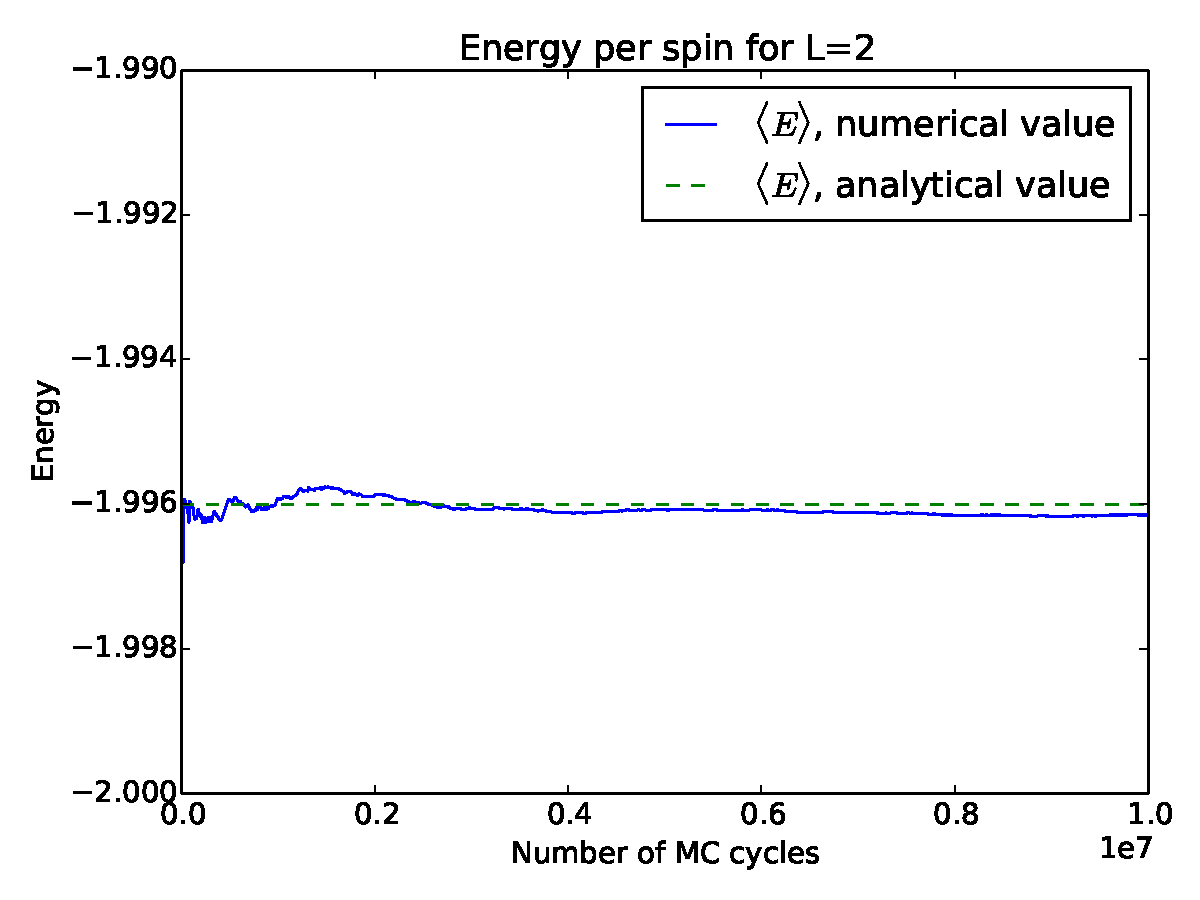
\includegraphics[width=1\linewidth]{../results/4b/L_2_energy}
\caption{Mean energy as a function of Monte Carlo cycles. }
\label{fig:l2energy}
	\end{subfigure}
	\hfill
	\begin{subfigure}[b]{0.49\textwidth}
	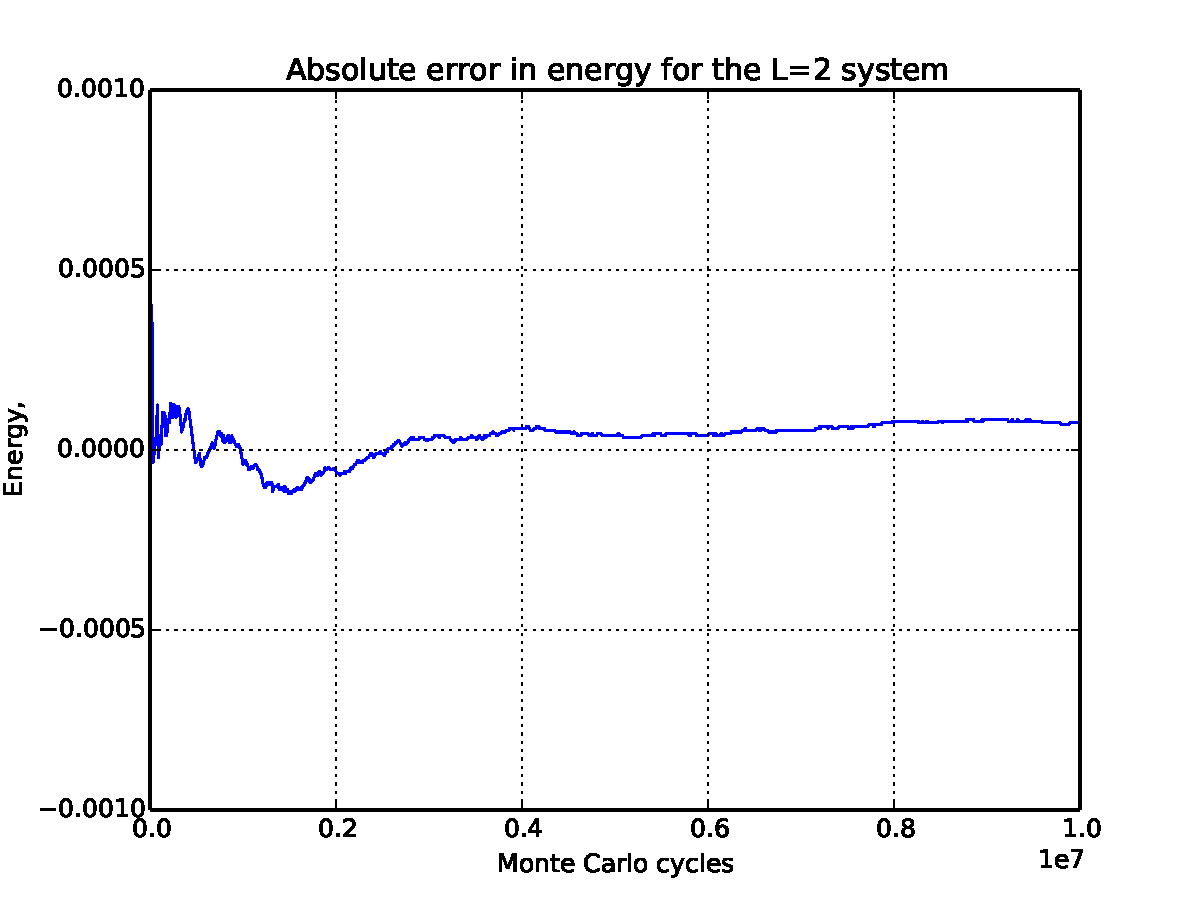
\includegraphics[width=1\linewidth]{../results/4b/abs_error}
\caption{Mean absolute error for the energy}
\label{fig:abserror}
	\end{subfigure}
	\caption{Mean energy and mean absolute error of the energy at $T=1 \frac{k_BT}{J}$.}
\end{figure}

\begin{figure}[H]
	\centering
	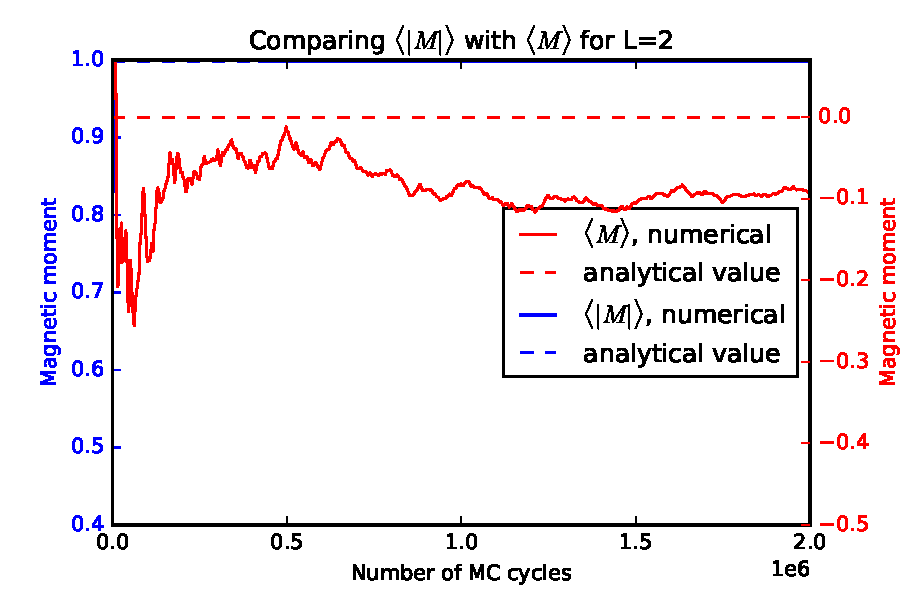
\includegraphics[width=0.7\linewidth]{../results/4b/L_2_mag_magabs}
	\caption{Comparison of the mean magnetization and the mean absolute magnetization. }
	\label{fig:l2magmagabs}
\end{figure}






Due to the smaller fluctuation of  $ \langle \abs{M} \rangle $, the susceptibility for the system was calculated by \begin{equation}
\chi = \frac{1}{k_B T} \left( 	\langle M^2 \rangle - \langle \abs{M}\rangle^2 	\right)\label{eq_X_def_new}
\end{equation}


	\begin{figure}[H]
		\begin{subfigure}[b]{0.49\textwidth}
	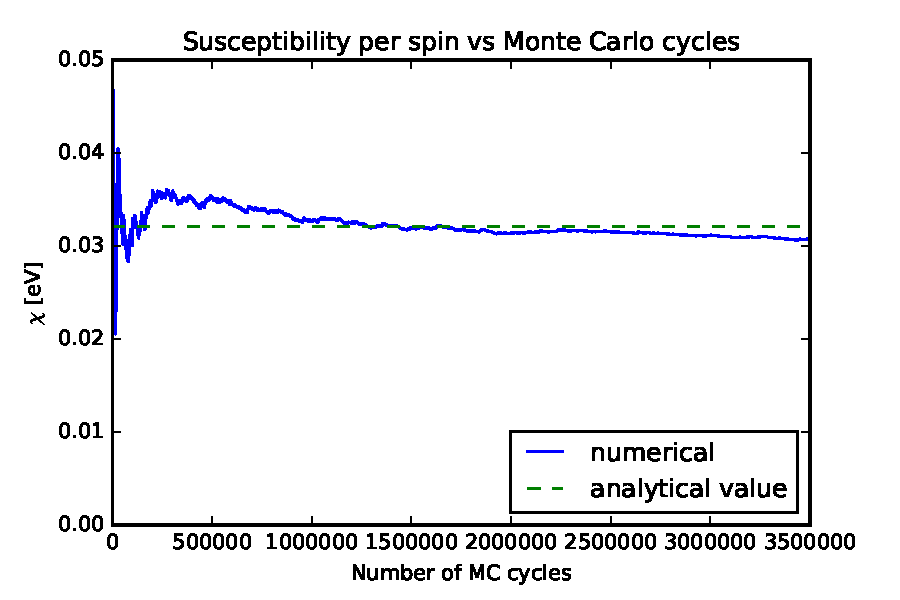
\includegraphics[width=1\linewidth]{../results/4b/L_2_susceptibility}
\caption{}
\label{fig:l2susceptibility}
		\end{subfigure}
		\hfill
		\begin{subfigure}[b]{0.49\textwidth}
		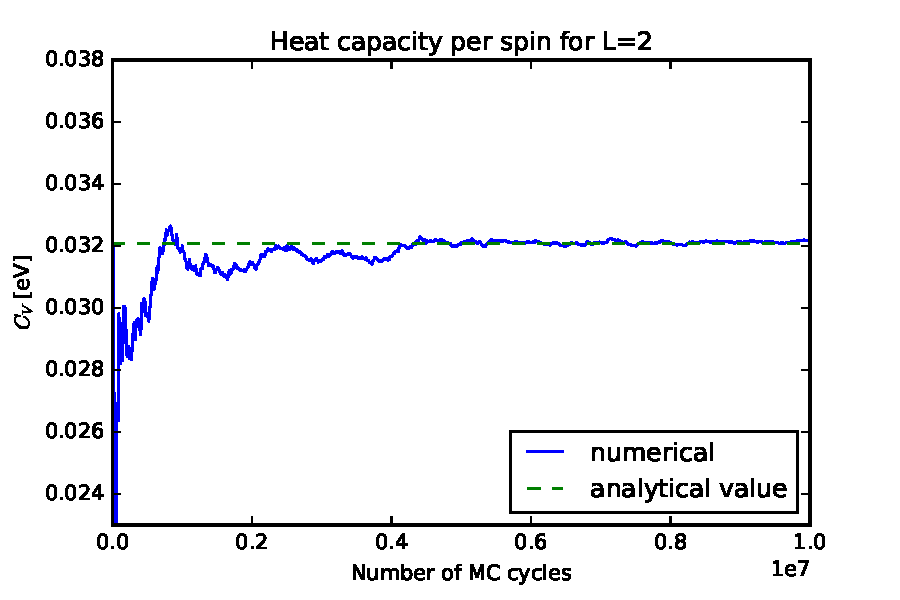
\includegraphics[width=1\linewidth]{../results/4b/L_2_heat_capasity}
\caption{}
\label{fig:l2heatcapasity}
		\end{subfigure}
		\caption{}
	\end{figure}



All calculations in this subsection are at T = 1.0 K. 

%\begin{table}[H]
%\caption{This table compares the analytical values for L=2 with the numerical ones after $10^6$ Monte Carlo cycles. The values are in units per spin.}\label{tab:compare_values}
%	\begin{tabular}{ccc}
%		& Numerical: & Analytical:\\ \hline
%		$\left<E\right>$ &   -1.9958 & -1.9960\\
%		$\left<E^2\right>$ &   15.9664 & 15.9679\\
%		$\left<M\right>$ &    0.0451 & 0\\
%		$\left<M^2\right>$ &    3.9930 & 3.9933\\
%		$\left<|M|\right>$ &    0.9986 & 0.9987\\
%		$\chi$ &   3.9849 & 3.9933\\
%		$C_V$& 0.0335 & 0.0321\\
%	\end{tabular}
%\end{table}


\subsection{The L=20 system}

HMM: Should define an area that is enough for equilibrium!

OBS: Need the number of MC cycles to reach equilibrium!

OBS: Need equilibration time! (5 1e5?)

OBS: Comment accepted configs T dependency


\subsubsection{Initial ordering of the system}






\begin{figure}[H]
	\begin{subfigure}[b]{0.49\textwidth}
	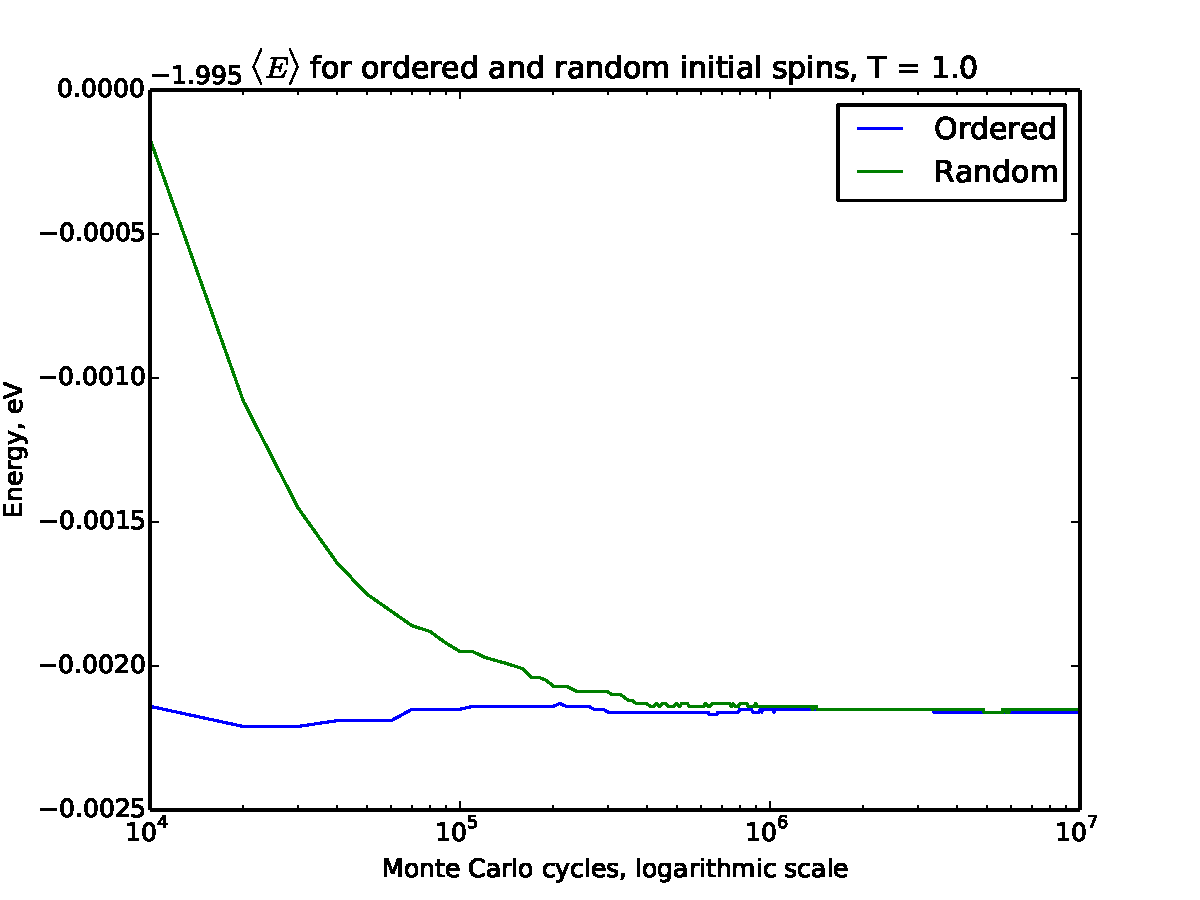
\includegraphics[width=1\linewidth]{../results/4c/ran_order_T1}
\caption{}
\label{fig:ranordert1}
	\end{subfigure}
	\hfill
	\begin{subfigure}[b]{0.49\textwidth}
	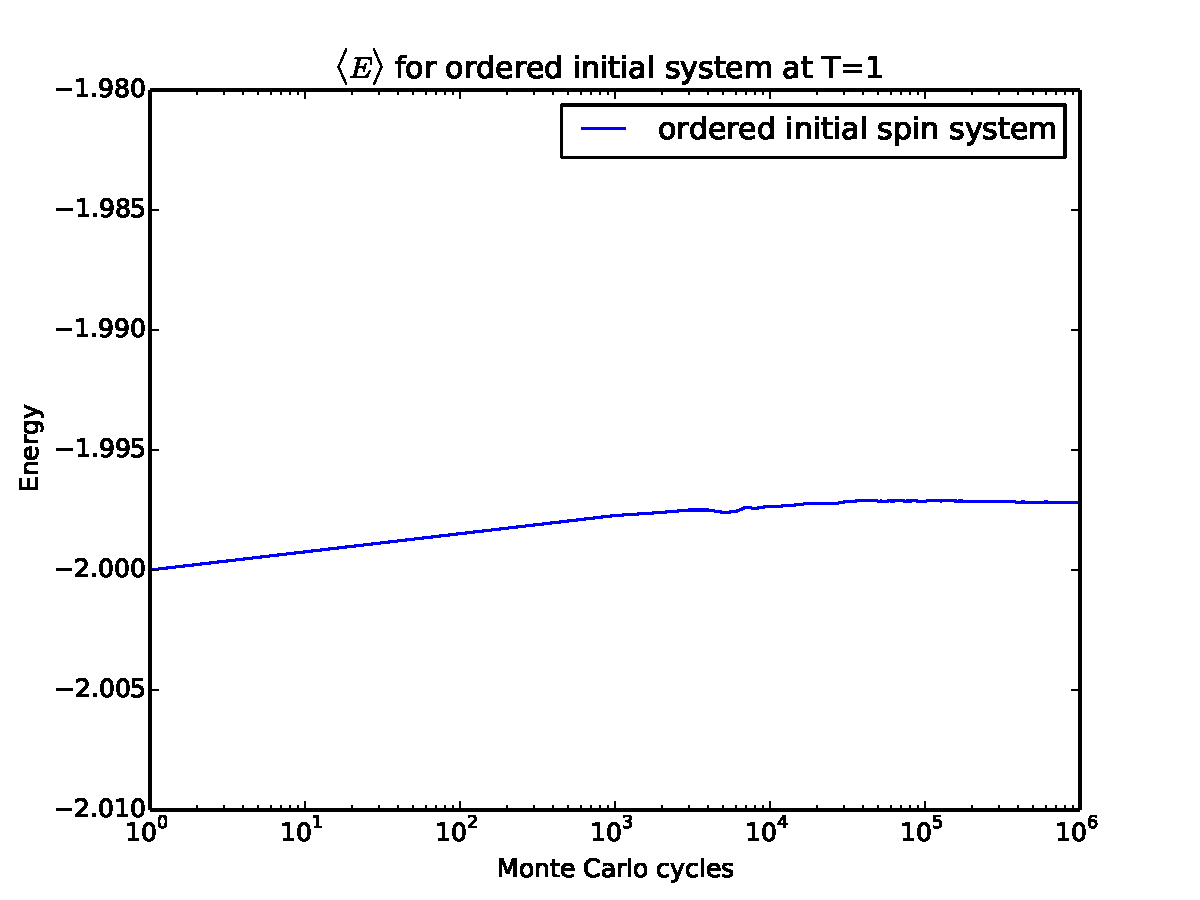
\includegraphics[width=1\linewidth]{../results/4c/order_T1_start}
\caption{}
\label{fig:ordert1start}
	\end{subfigure}
	\caption{}
\end{figure}











\begin{figure}[H]
	\centering
	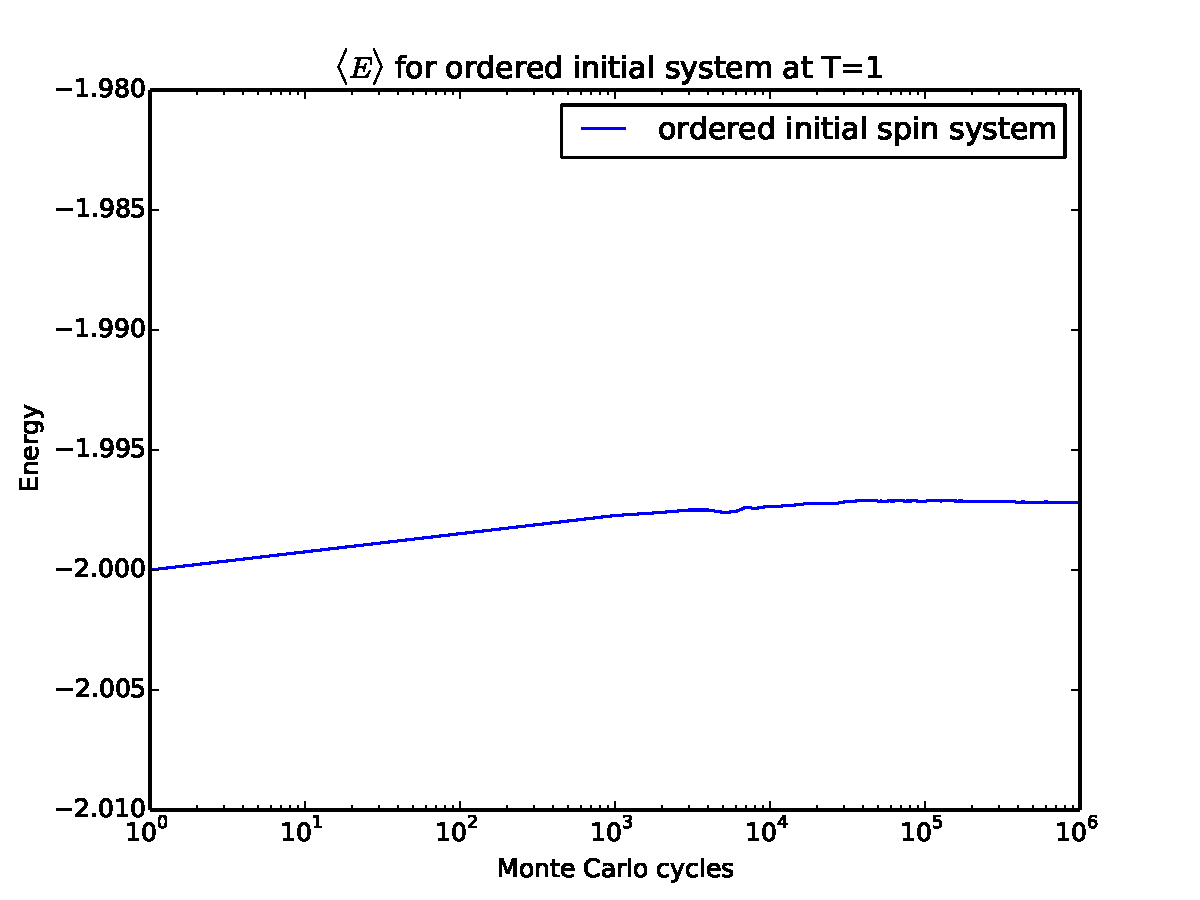
\includegraphics[width=0.7\linewidth]{../results/4c/order_T1_start}
	\caption{ Plot of the  }
	\label{fig:ranorder_t1_start}
\end{figure}
\begin{figure}[H]
		\centering
	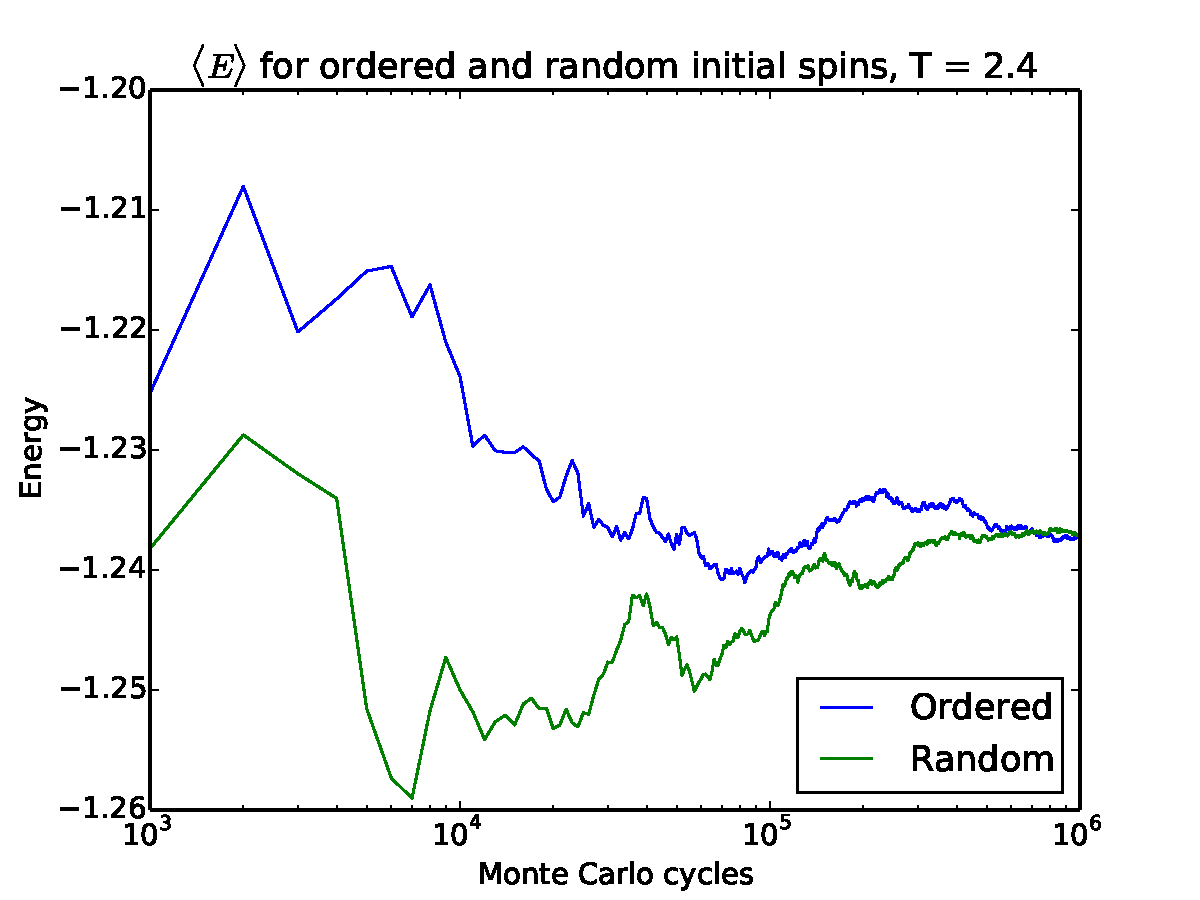
\includegraphics[width=0.7\linewidth]{../results/4c/ran_order_T2}
	\caption{}
	\label{fig:ranordert2}
\end{figure}






\subsubsection{Equilibrium time  for the random L=20 system}





	\begin{figure}[H]
	\begin{subfigure}[b]{0.49\textwidth}
		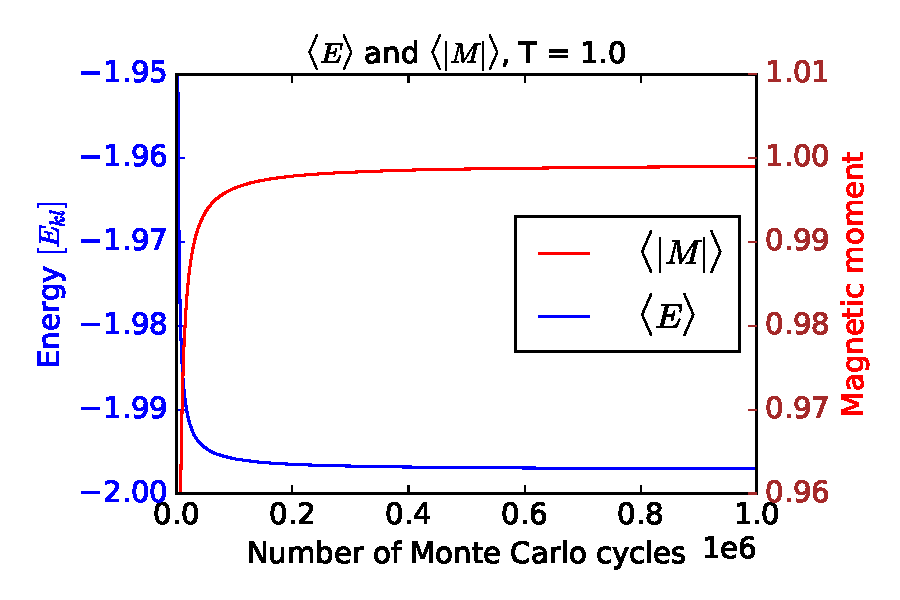
\includegraphics[width=1\linewidth]{../results/4c/En_mag_T1_0}
		\caption{}
		\label{fig:L20_mag_T_1}
	\end{subfigure}
	\hfill
	\begin{subfigure}[b]{0.49\textwidth}
		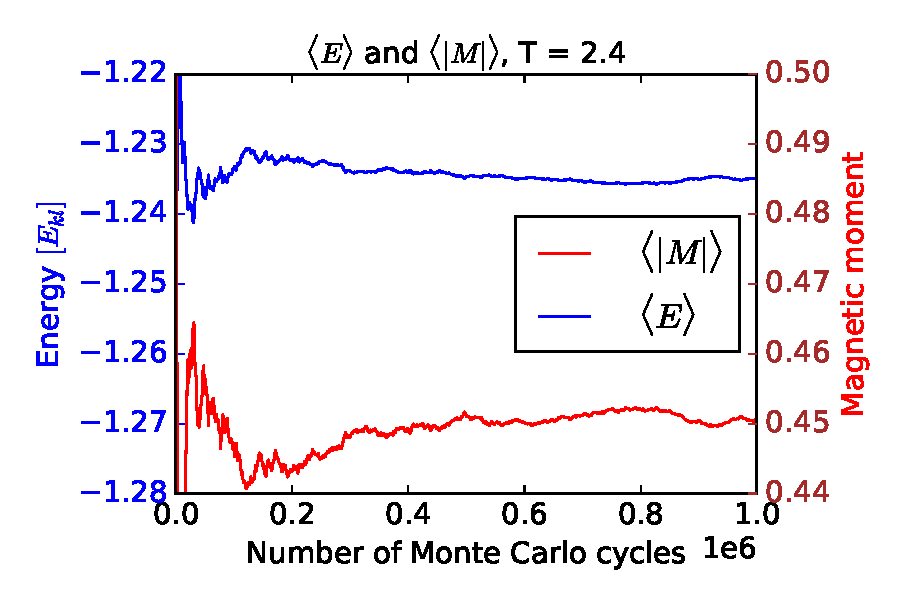
\includegraphics[width=1\linewidth]{../results/4c/En_mag_T2_4}
		\caption{}
		\label{fig:L20_mag_T_2-4}
	\end{subfigure}
	\caption{}
\end{figure}




	\begin{figure}[H]
	\begin{subfigure}[b]{0.49\textwidth}
	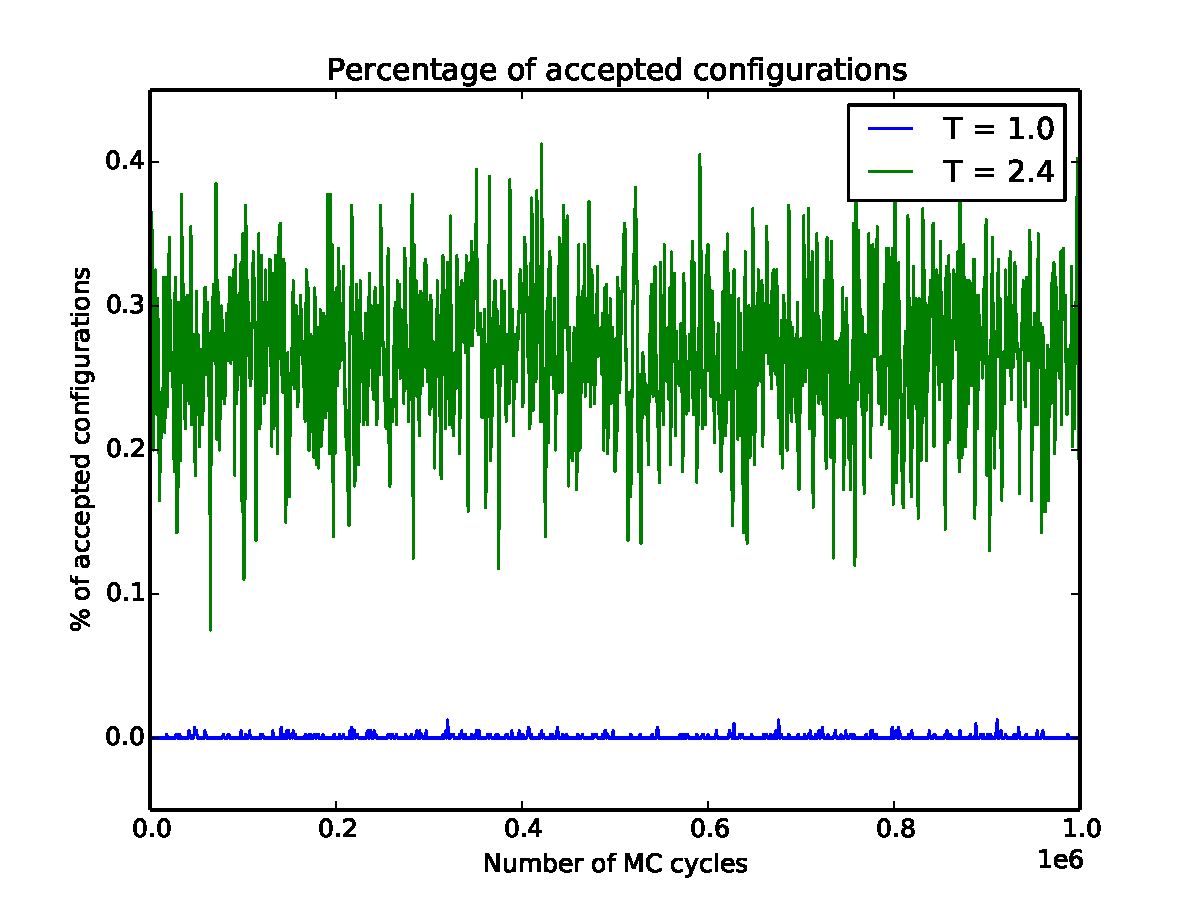
\includegraphics[width=1\linewidth]{../results/4c/L_20_accepted_configs}
\caption{}
\label{fig:l20acceptedconfigs}
	\end{subfigure}
	\hfill
	\begin{subfigure}[b]{0.49\textwidth}
	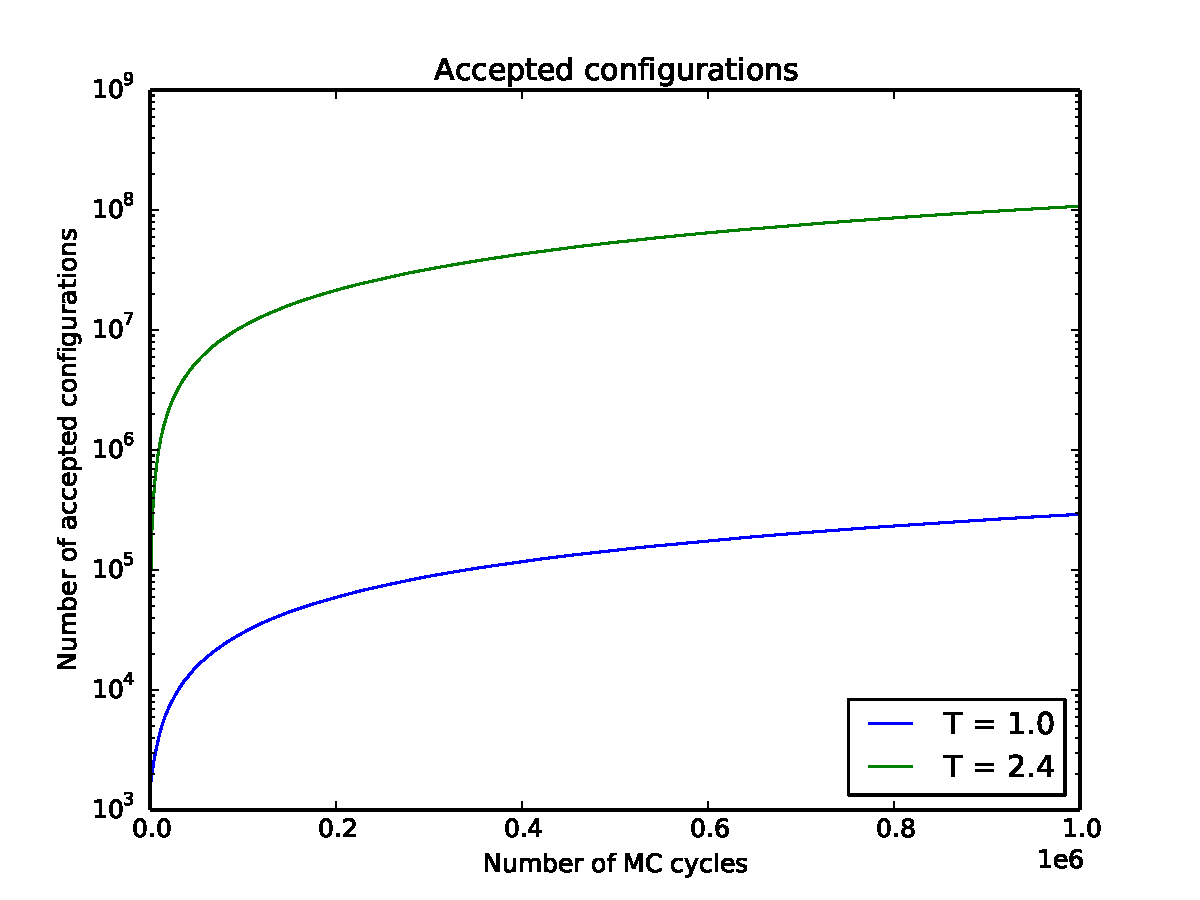
\includegraphics[width=1\linewidth]{../results/4c/L_20_accepted_configs_}
\caption{}
\label{fig:l20acceptedconfigs}
	\end{subfigure}
	\caption{}
\end{figure}











\subsubsection{Probability distrubition  for the L=20 system}


OBS: Compare result with computed variance!

OBS: Discuss behavior (In Discussion - maybe just merge result and discussion?)

Computed variance (from same dataset?):

$$ \sigma_E^2 = \left< E^2\right> - \left< E\right>^2 $$

T = 1.0 K:

$$ \sigma_E^2 = 1595.45 - (-1.997)^2 = 1591.46$$

T = 2.4 K:

$$ \sigma_E^2 =   620.734 - (-1.23759)^2
= 619.20$$



\begin{figure}[H]
	\centering
	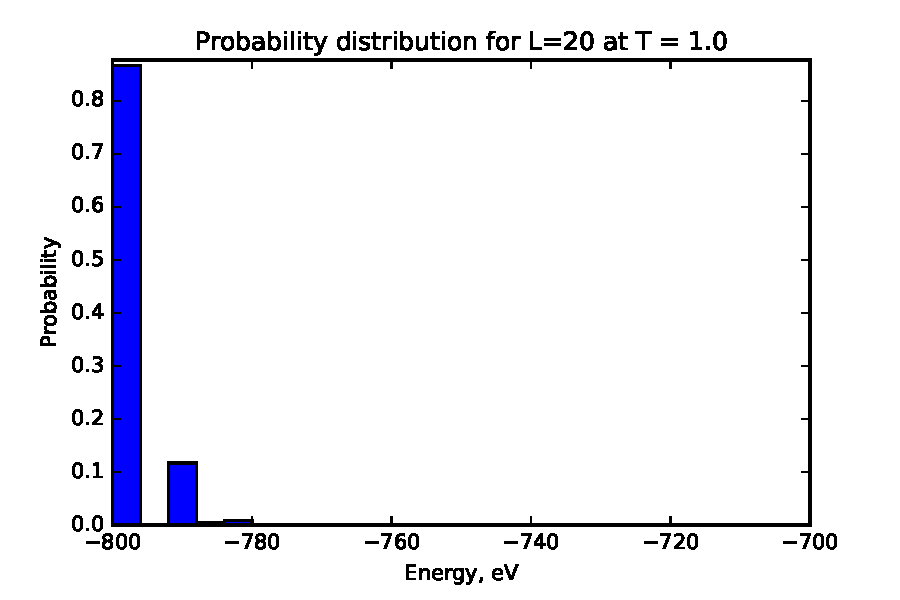
\includegraphics[width=0.7\linewidth]{../results/4d/PD_T_1MC_1e6}
	\caption{}
	\label{fig:pdt1}
\end{figure}

\begin{figure}[H]
	\centering
	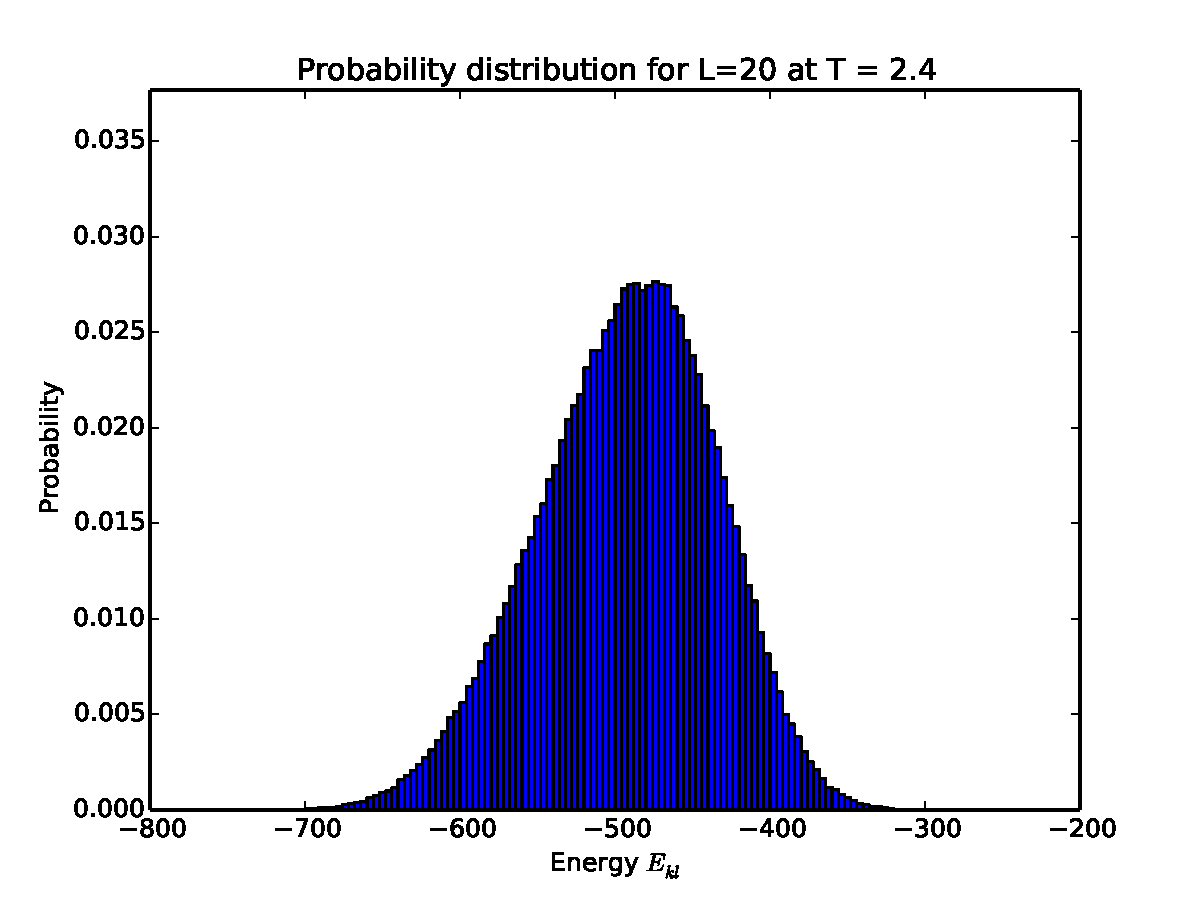
\includegraphics[width=0.7\linewidth]{../results/4d/PD_T_2MC_1e6}
	\caption{}
	\label{fig:pdt2_4}
\end{figure}



\subsection{Phase transition and Critical temperature}



OBS: Plot of E, M, Cv, X as functions of T (put L as legend and plot together)

OBS: Indication of phase transition? (Peak - at least for Cv and X)

OBS: Use Equation \ref{eq:critical_T} to extract $T_C$.


Timing parallellisering

	\begin{figure}[H]
	\begin{subfigure}[b]{0.5\textwidth}
	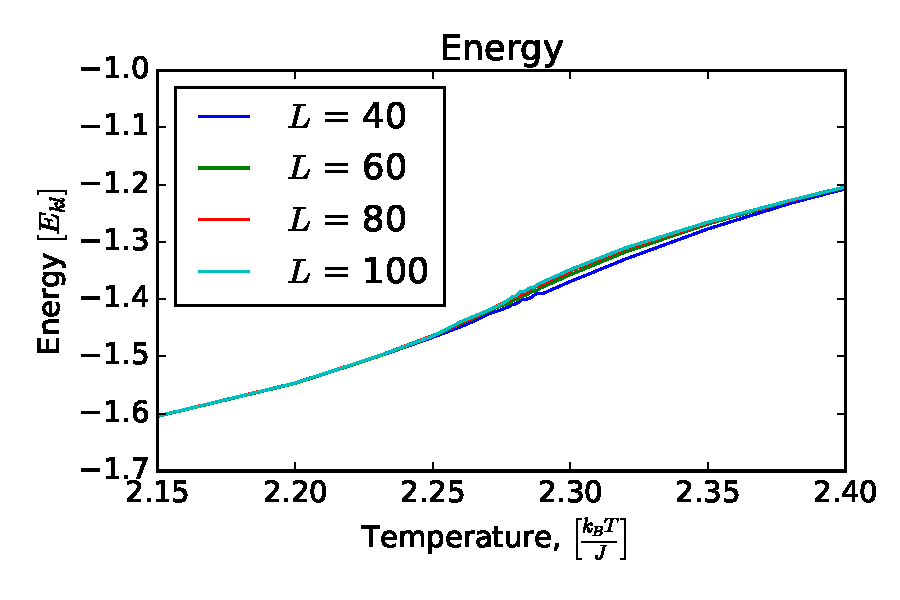
\includegraphics[width=1\linewidth]{../results/4e/4e_energy}
\caption{}
\label{fig:4eenergy}
	\end{subfigure}
	\hfill
	\begin{subfigure}[b]{0.5\textwidth}
	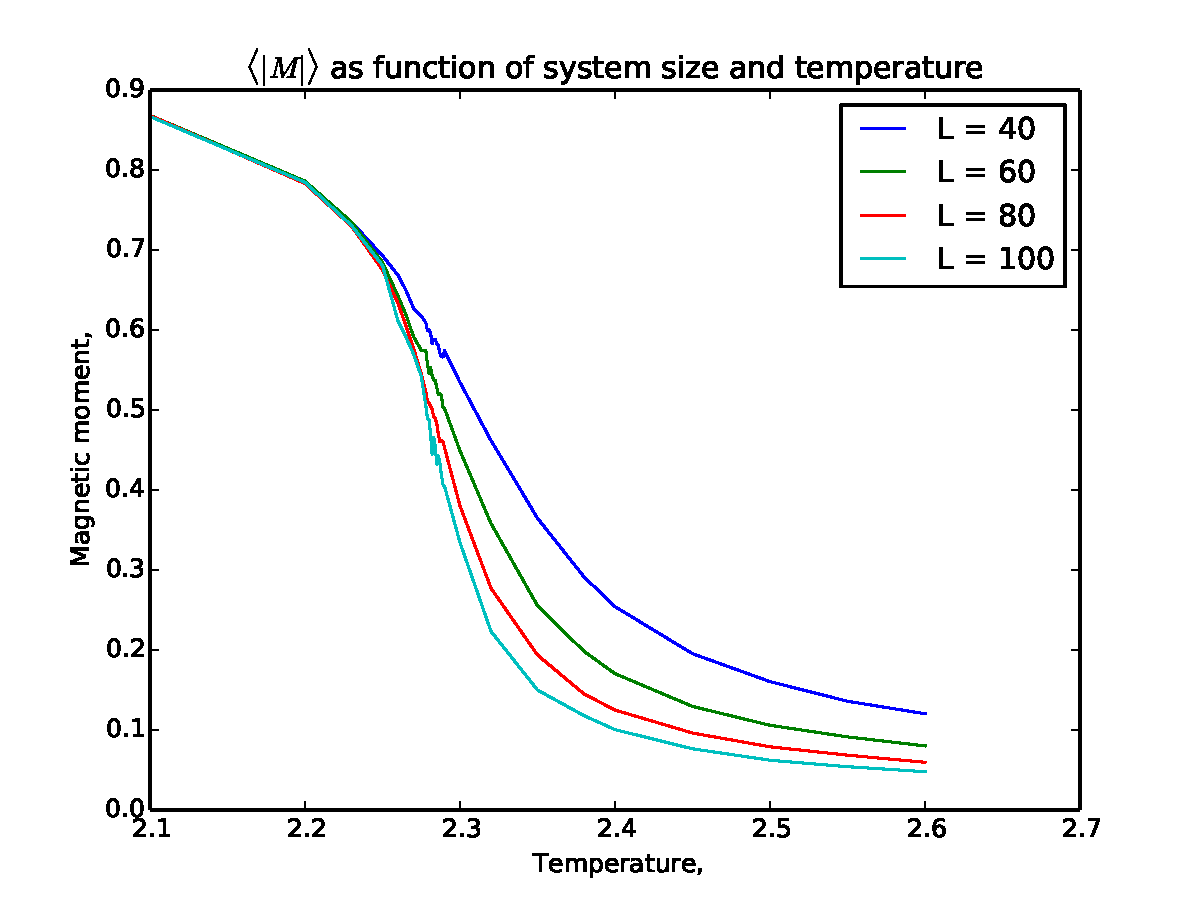
\includegraphics[width=1\linewidth]{../results/4e/4e_mag}
\caption{}
\label{fig:4emag}
	\end{subfigure}
	\caption{}
\end{figure}




\begin{figure}[H]
	\centering
	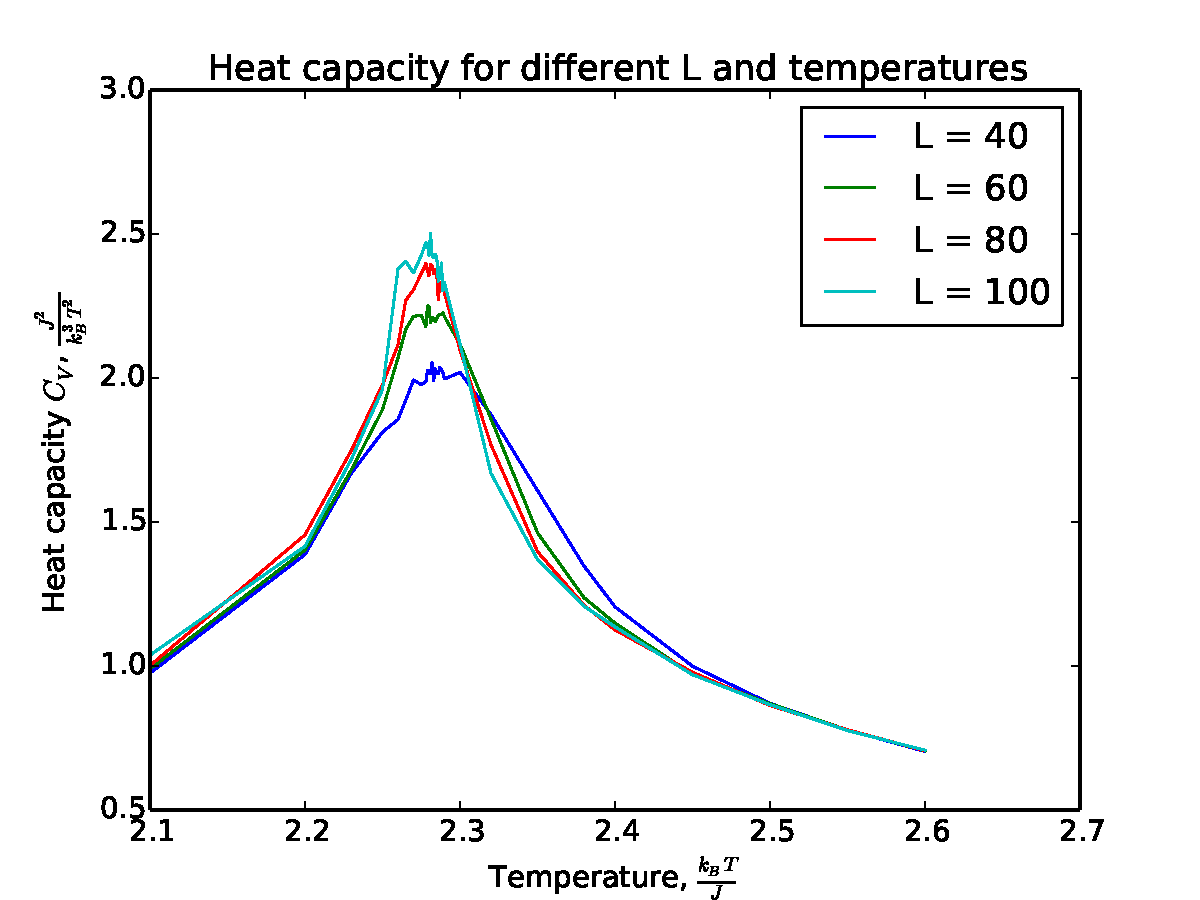
\includegraphics[width=0.7\linewidth]{../results/4e/4e_Cv}
	\caption{}
	\label{fig:4ecv}
\end{figure}

\begin{figure}[H]
	\centering
	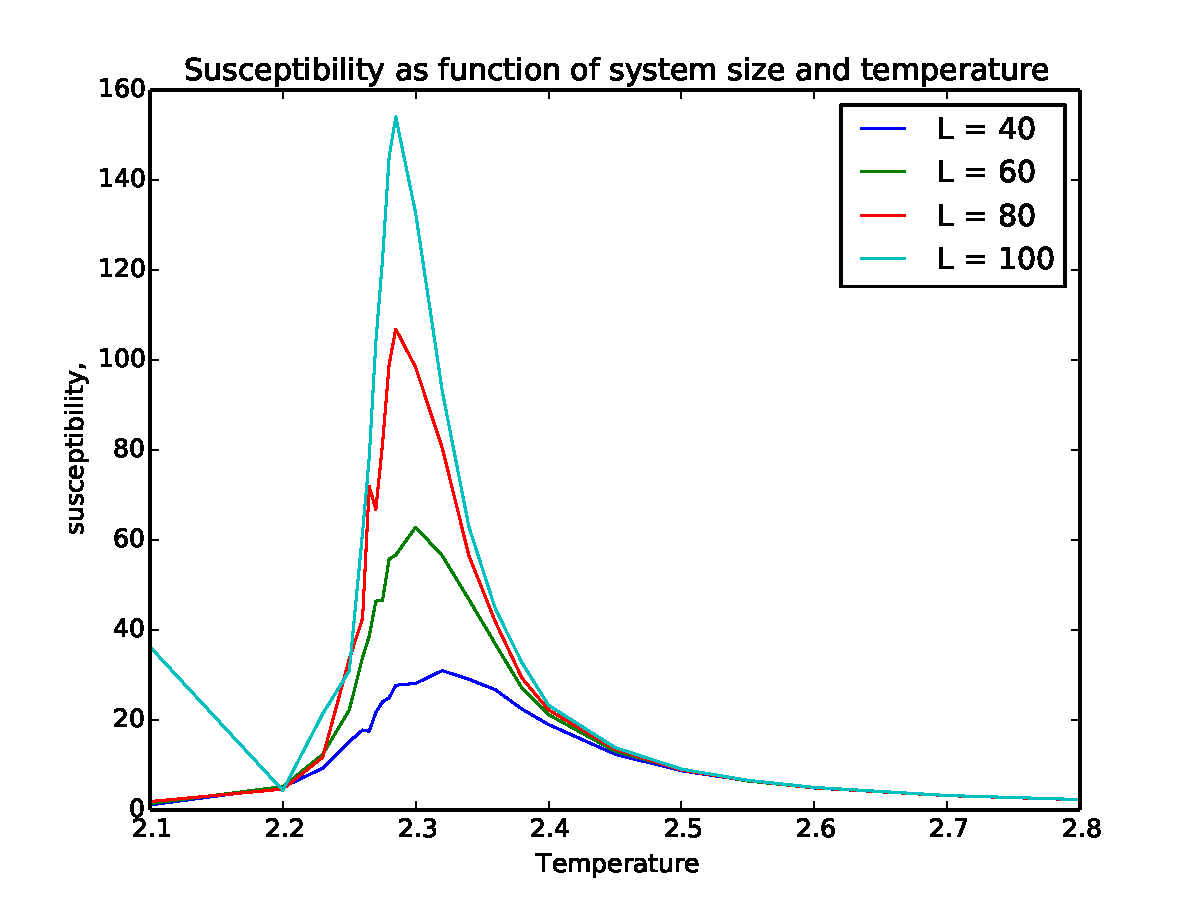
\includegraphics[width=0.7\linewidth]{../results/4e/4e_x}
	\caption{}
	\label{fig:4ex}
\end{figure}


\begin{table}[H]
	\caption{text}
	\label{tab: T_C}
	\begin{tabular}{cccccc}
		 L & $T_C$ \\ \hline    
     40 & 2.282 \\ 
 60 & 2.279 \\ 
 80 & 2.278 \\ 
 100 & 2.281 \\ 

	\end{tabular}
\end{table}




Exact $T_C =  kTC/J = 2/ \ln(1+\sqrt{
	2}) \approx 2.269$ \cite{Onsager}

\begin{table}\caption{L=80 and MC cycles is 1e6.}
	\begin{tabular}{cc}
		Number of processors:& CPU time [s]: \\ \hline
		1 & 513.069\\
		2 & 306.975\\
	\end{tabular}
\end{table}
